\documentclass[12pt,letterpaper]{article}

\usepackage[margin=1in]{geometry}
\usepackage[group-separator={,},round-mode=figures,round-precision=3,scientific-notation=false]{siunitx}
\usepackage[super]{nth}
\usepackage[title]{appendix}
\usepackage{amsfonts}
\usepackage{amsmath}
\usepackage{amsthm}
\usepackage{cancel}
\usepackage{caption}
\usepackage{color, colortbl}
\usepackage{dcolumn}
\usepackage{enumitem}
\usepackage{fp}
\usepackage{float}
\usepackage{listings}
\usepackage{mathtools}
\usepackage{pgfplots}
\usepackage{subcaption}
\usepackage{systeme}
\usepackage{tikz}
\usepackage{titling}

\usepgfplotslibrary{statistics}

\usetikzlibrary{intersections}
\usetikzlibrary{patterns}

\pgfplotsset{compat=1.8}

\definecolor{Gray}{gray}{0.8}
\newcolumntype{g}{>{\columncolor{Gray}}c}
\newcolumntype{d}{D{.}{.}{-1}}
\DeclarePairedDelimiter\ceil{\lceil}{\rceil}
\DeclarePairedDelimiter\floor{\lfloor}{\rfloor}

\newcommand*\circled[1]{%
  \tikz[baseline=(char.base)]{
    \node[shape=circle,draw,inner sep=2pt] (char) {#1};
  }
}

\makeatletter
\renewcommand*\env@matrix[1][*\c@MaxMatrixCols c]{%
  \hskip -\arraycolsep
  \let\@ifnextchar\new@ifnextchar
  \array{#1}}
\makeatother

\newcommand*\constant[1]{%
  Each product has a different #1,
  but these are constant values not constrained by anything else in the process.
}

\newcommand*\genericconstraint[2]{%
  Each product has a #1 constraint on #2.
}

\newcommand*\maximumconstraint[1]{%
  \genericconstraint{maximum}{#1}
}

\newcommand*\minimumconstraint[1]{%
  \genericconstraint{minimum}{#1}
}

\newcommand*\genericobjective[2]{%
  The objective is to #1 #2.
}

\newcommand*\maximumobjective[1]{%
  \genericobjective{maximum}{#1}
}

\newcommand*\minimumobjective[1]{%
  \genericobjective{minimum}{#1}
}

\newcommand*\buck[1]{%
  \$\num{#1}%
}

\lstdefinelanguage{zimpl}{
  morekeywords={forall,in,maximize,minimize,param,set,subto,sum,var},
  sensitive=true,
  morecomment=[l]{\#},
  morestring=[b]",
}
\lstset{basicstyle=\scriptsize, frame=single, language=zimpl}

\setlength{\droptitle}{-10ex}

\preauthor{\begin{flushright}\large \lineskip 0.5em}
\postauthor{\par\end{flushright}}
\predate{\begin{flushright}\large}
\postdate{\par\end{flushright}}

\title{MAT 168 Modeling 3\vspace{-2ex}}
\author{Hardy Jones\\
        999397426\\
        Professor K\"{o}ppe\vspace{-2ex}}
\date{Spring 2015}

\begin{document}
  \maketitle

  \begin{enumerate}
    \setcounter{enumi}{2}
    \item
      \begin{enumerate}
        \item
          After modifying the given ZIMPL file and running it on all 14 tours,
          we can compare to the optimal:

          \begin{tabular}{l | r | r | r}
            \hline
            \hline
            Tour      & Optimal & Nearest Neighbor & Subtours \\
            \hline
            a280      & 2579    & 3157             & 2550     \\
            ali535    & 202310  & 265685           & 193429   \\
            berlin52  & 7542    & 8980             & 7164     \\
            burma14   & 3323    & 4501             & 3001     \\
            gr137     & 69853   & 98781            & 67009    \\
            gr202     & 40160   & 54092            & 38576    \\
            gr229     & 134602  & 162109           & 128353   \\
            gr431     & 171414  & 206628           & 163905   \\
            gr666     & 294358  & 364429           & 286428   \\
            gr96      & 55209   & 74939            & 53069    \\
            pr226     & 80369   & 94683            & 57177    \\
            u574      & 36905   & 50459            & 34422    \\
            ulysses16 & 6859    & 8081             & 6113     \\
            ulysses22 & 7013    & 8248             & 6160     \\
            \hline
          \end{tabular}

          What we see is that every solution is more optimal than the optimal solution.
        \item
          See Figure \ref{fig:burma1401}

          \begin{figure}
            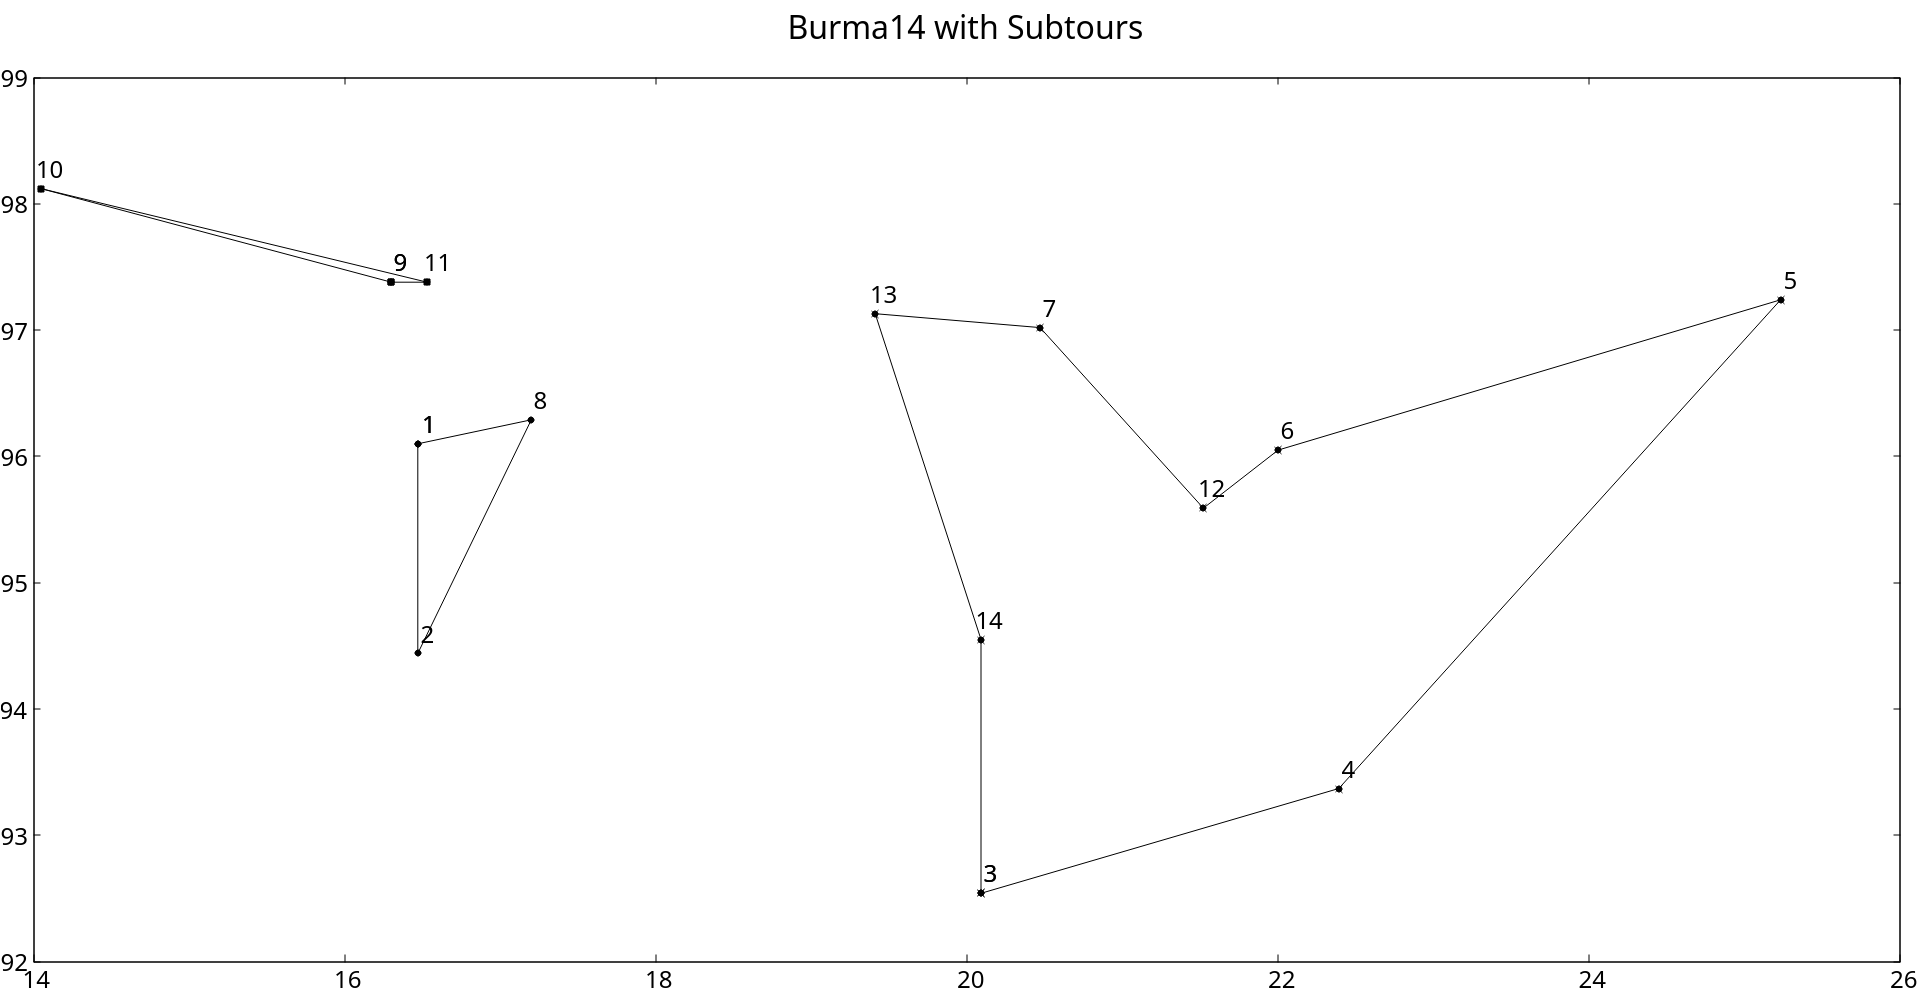
\includegraphics[width=\textwidth]{distances/burma14_subtours_0_1.png}
            \caption{Visualization of \texttt{burma14Distances.txt}}
            \label{fig:burma1401}
          \end{figure}

        \item
          After changing the variables to real values between 0 and 1, we now have these results:

          \begin{tabular}{l | r | r | r | r}
            \hline
            \hline
            Tour      & Optimal & Nearest Neighbor & Subtours & Subtours Fractional \\
            \hline
            a280      & 2579    & 3157             & 2550     & 2534                \\
            ali535    & 202310  & 265685           & 193429   & 191454.5            \\
            berlin52  & 7542    & 8980             & 7164     & 7163                \\
            burma14   & 3323    & 4501             & 3001     & 3001                \\
            gr137     & 69853   & 98781            & 67009    & 66643.5             \\
            gr202     & 40160   & 54092            & 38576    & 38383.5             \\
            gr229     & 134602  & 162109           & 128353   & 127411              \\
            gr431     & 171414  & 206628           & 163905   & 163027              \\
            gr666     & 294358  & 364429           & 286428   & 284803.5            \\
            gr96      & 55209   & 74939            & 53069    & 52728.5             \\
            pr226     & 80369   & 94683            & 57177    & 55247.5             \\
            u574      & 36905   & 50459            & 34422    & 34256               \\
            ulysses16 & 6859    & 8081             & 6113     & 6113                \\
            ulysses22 & 7013    & 8248             & 6160     & 6106.5              \\
            \hline
          \end{tabular}

          The first thing to notice is that each example runs much quicker.
          Since we have relaxed the problem, this should not be a surprise.

          We also see that most of the tours now have slightly more optimal solutions than before.
      \end{enumerate}
    \item
      \begin{enumerate}
        \item
          After modifying the model to eliminate subtours,
          only two tours can be computed.
          The other tours consume too much memory to complete and are killed by the OS.

          The two tours are \texttt{burma14} and \texttt{ulysses16}--with \texttt{ulysses16} being the larger tour.
          And both of these tours have the optimal solution of 3323 and 6859 respectively.

          See Figure \ref{fig:ulysses16elimination}

          \begin{figure}
            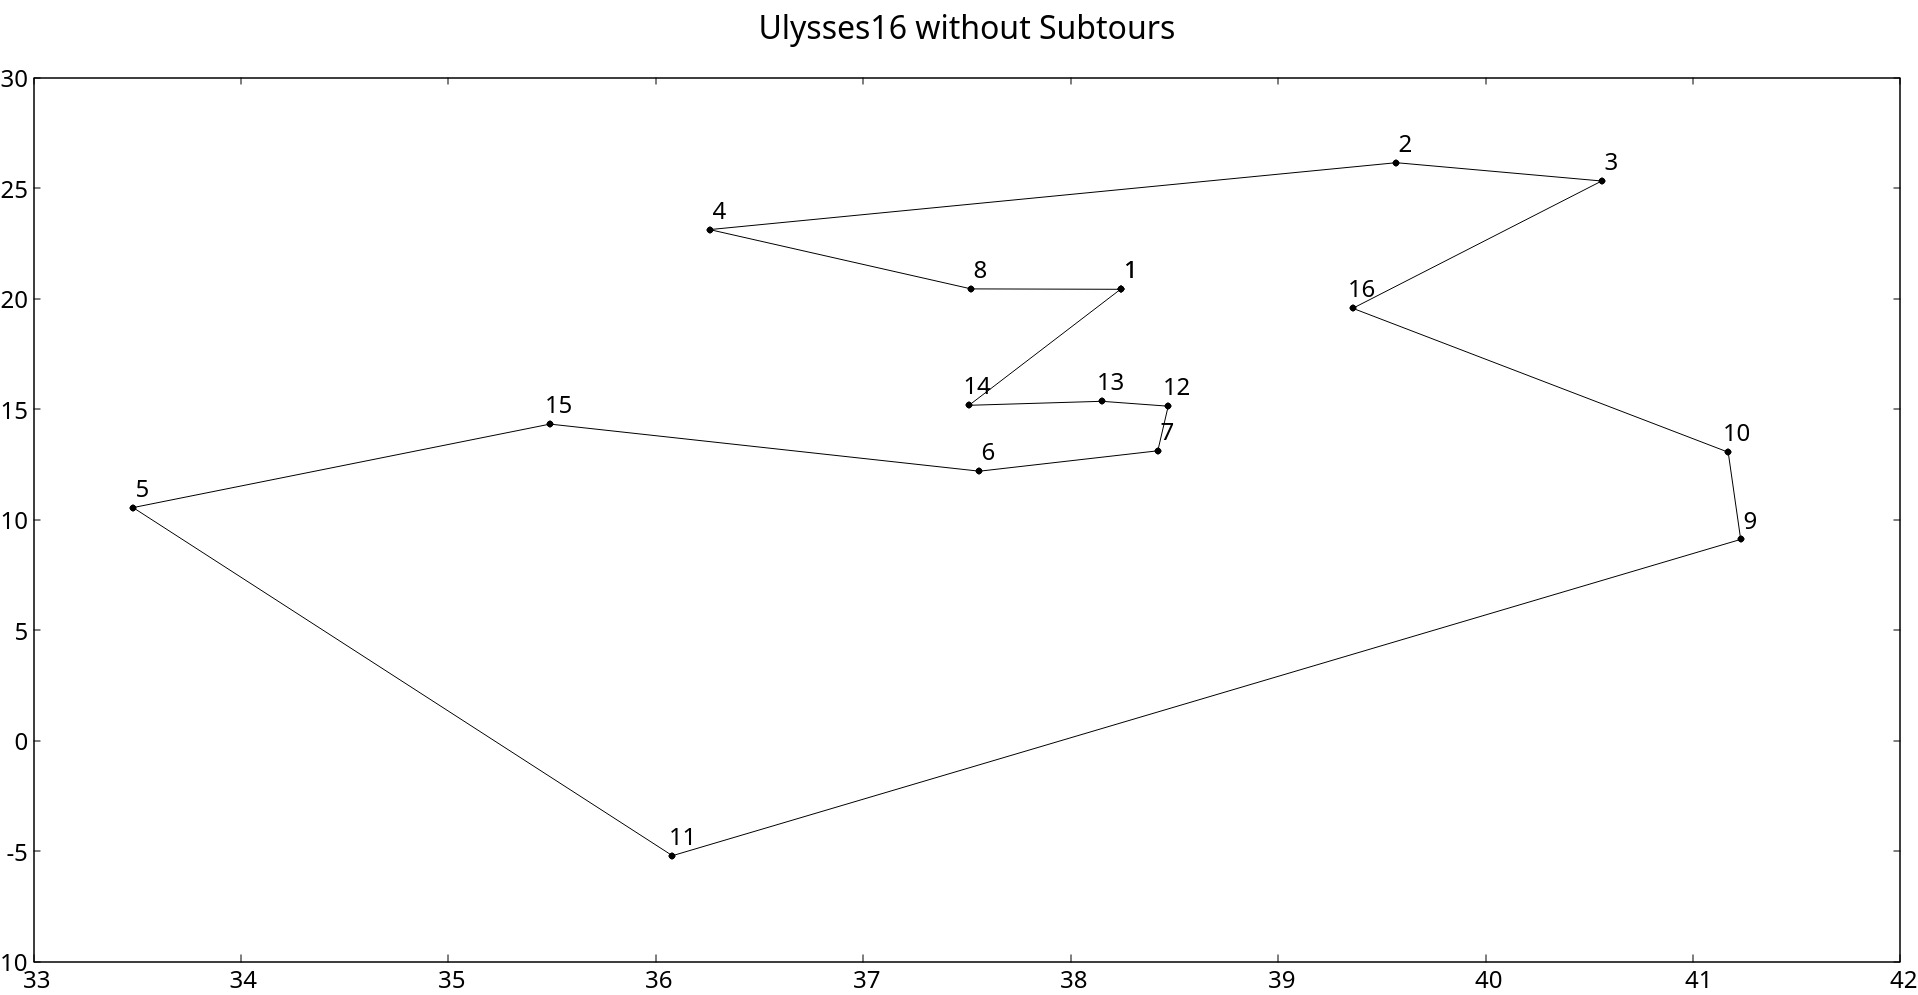
\includegraphics[width=\textwidth]{distances/ulysses16_subtours_elimination_0_1.png}
            \caption{Visualization of \texttt{ulysses16} without subtours}
            \label{fig:ulysses16elimination}
          \end{figure}

        \item
          Again, we can only run the two tours \texttt{burma14} and \texttt{ulysses16}.

          Interestingly the tours generated are the same, so we eschew visualizing the same tours.
      \end{enumerate}
    \item
      Yet again we are restricted to \texttt{burma14} and \texttt{ulysses16}.
      In each of the cases, what we find is that the $k$ doesn't make a difference on the outcome.

      We can add this information to the table.

      \begin{tabular}{l | r | r | r | r | r}
        \hline
        \hline
        Tour      & Opt.    & N. N.            & Subtours & Subtours Fractional & $k \in \{3, 4, 5\}$ \\
        \hline
        a280      & 2579    & 3157             & 2550     & 2534                & N/A                 \\
        ali535    & 202310  & 265685           & 193429   & 191454.5            & N/A                 \\
        berlin52  & 7542    & 8980             & 7164     & 7163                & N/A                 \\
        burma14   & 3323    & 4501             & 3001     & 3001                & 3098                \\
        gr137     & 69853   & 98781            & 67009    & 66643.5             & N/A                 \\
        gr202     & 40160   & 54092            & 38576    & 38383.5             & N/A                 \\
        gr229     & 134602  & 162109           & 128353   & 127411              & N/A                 \\
        gr431     & 171414  & 206628           & 163905   & 163027              & N/A                 \\
        gr666     & 294358  & 364429           & 286428   & 284803.5            & N/A                 \\
        gr96      & 55209   & 74939            & 53069    & 52728.5             & N/A                 \\
        pr226     & 80369   & 94683            & 57177    & 55247.5             & N/A                 \\
        u574      & 36905   & 50459            & 34422    & 34256               & N/A                 \\
        ulysses16 & 6859    & 8081             & 6113     & 6113                & 6228                \\
        ulysses22 & 7013    & 8248             & 6160     & 6106.5              & N/A                 \\
        \hline
      \end{tabular}


      For the sake of brevity we only visualize one tour.

      See Figure \ref{fig:ulysses16eliminationk}

      \begin{figure}
        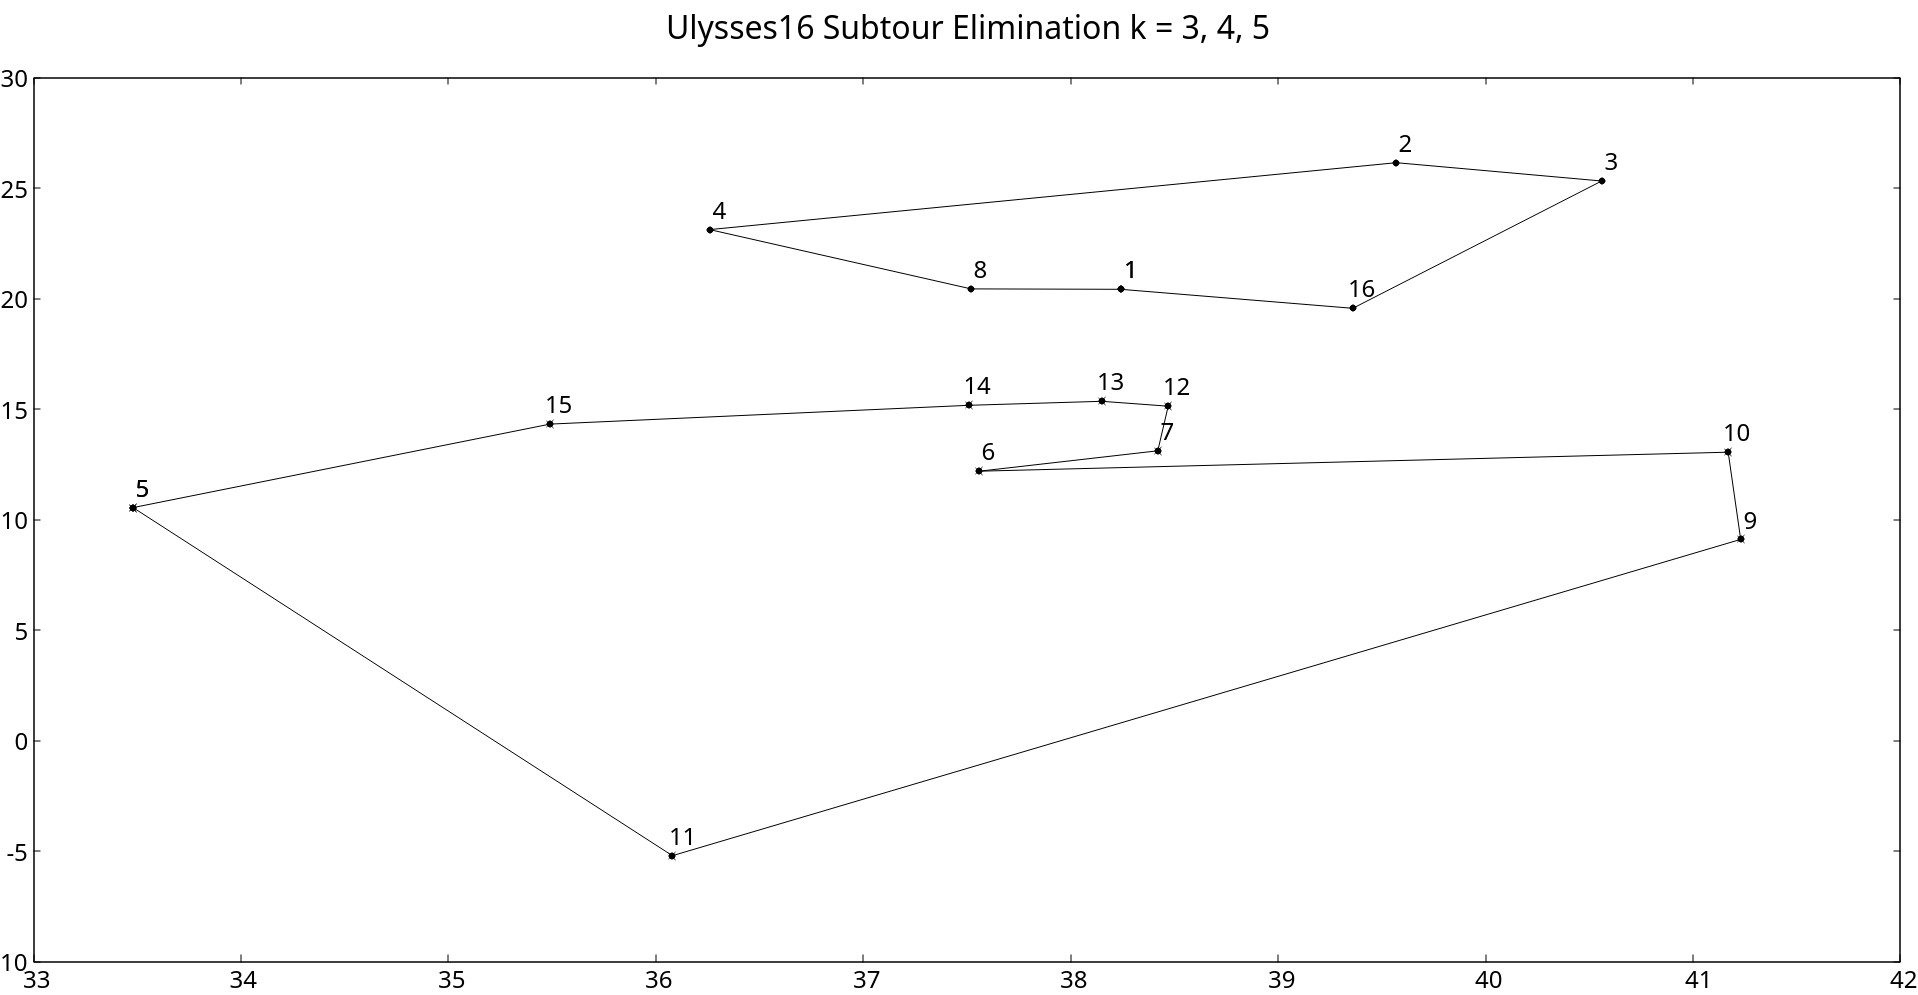
\includegraphics[width=\textwidth]{distances/ulysses16_subtours_elimination_k.png}
        \caption{Visualization of \texttt{ulysses16} without subtours for k = 3, 4, 5}
        \label{fig:ulysses16eliminationk}
      \end{figure}
  \end{enumerate}

  \pagebreak

  \begin{appendices}
    \section{ZIMPL}
      For each of the modeling files,
      we use a simple shell script to run them.

      This allows a decent interface that allows injecting a filename without manually manipulating the files.
      Each is a slight modification of the following format.

      \lstinputlisting[language=sh]{distances/subtours_0_1.sh}

      For problem 3a we use the following model:

      \lstinputlisting{distances/subtours_0_1.tmpl.zpl}

      For problem 3c we use the following model:

      \lstinputlisting{distances/subtours_fractional.tmpl.zpl}

      For problem 4a we use the following model:

      \lstinputlisting{distances/subtours_elimination_0_1.tmpl.zpl}

      For problem 4b we use the following model:

      \lstinputlisting{distances/subtours_elimination_fractional.tmpl.zpl}

      \pagebreak

      For problem 5 we use the following model:

      \lstinputlisting{distances/subtours_elimination_fractional_3.tmpl.zpl}

      For sake of brevity, we just show one model for $k = 3$.
      The other models are similar with the value of $k$ changed.
  \end{appendices}
\end{document}
